%\def\newblock{\hskip .11em plus .33em minus .07em}

\documentclass{llncs}
\usepackage{graphicx}
\sloppy

\usepackage{amssymb}
\usepackage{amsmath}
\usepackage{graphicx}
\usepackage{epsfig}
\usepackage{subfigure}
\usepackage{listings}
\usepackage{verbatim}
\usepackage[T1]{fontenc} 
\usepackage{url}
\lstset{language=ml}
\lstset{commentstyle=\textit}
\lstset{mathescape=true}
\lstset{backgroundcolor=,rulecolor=}
\lstset{frame=single}
\lstset{breaklines=true}
\lstset{basicstyle=\ttfamily \small}

\newcommand{\Nat}{{\mathbb N}}
\newcommand{\Real}{{\mathbb R}}

\begin{document}

\title{Monadic Scripting in F\# for Computer Games}

\author{
G. Maggiore, \ M. Bugliesi, \ R. Orsini
  \institute{Universit\`a Ca' Foscari Venezia \\
  \email{\{maggiore,bugliesi,orsini\}@dais.unive.it}
}
}

\maketitle

\date{}

\begin{abstract}
Modern game architectures provide for a clean separation between
game engine and game content, making engines \textit{scriptable}, so
as to delegate the development of the main functionalities related to
gameplay to scripts coded in high-level languages. 

Game scripting poses two orders of problems. First, the scripting
language must be equipped with coroutining mechanisms to support a
smooth interaction between the discrete-time structure of the game
animation implemented by the engine with the execution of the
scripts, which typically implement character behavior spanning 
multiple simulation ticks. Secondly, these mechanisms should be transparent, to
ease design and development, and at the same time offer the highest
run-time performance to keep up with the interactive frameratess
expected by the user. 

We present a monadic framework that elegantly solves these problems
and compare it with the most commonly used systems, and discuss how it has
been integrated in actual projects. 
\end{abstract}

\keywords{games, monadic programming, state management, scripting}

\section{Introduction}
\label{sec:intro}
%%%%%%%%%%%%%%%%%%%%%%%%%%%%%%%%%%%%%%%%%%%%%%%%%%%%%%%%%%
% intro.tex
%%%%%%%%%%%%%%%%%%%%%%%%%%%%%%%%%%%%%%%%%%%%%%%%%%%%%%%%%%


\begin{figure}
\begin{center}
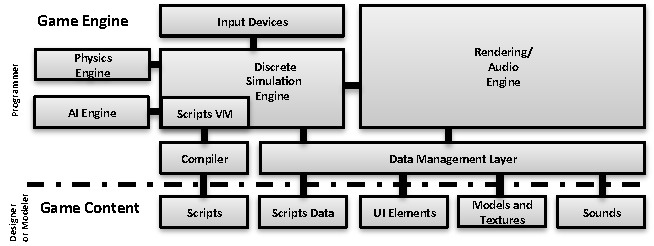
\includegraphics[scale=0.8]{engine_architecture.pdf}
\end{center}
\label{fig:data_driven_games}
\caption{Data-driven engine architecture, from \cite{SGL}}
\end{figure}

Virtual reality browsers face big challenges centered on performance and complexity. Performance is needed because the framerate at which the virtual world is rendered and animated must be high enough to give the user a feeling of smoothness. The scene must be rendered at least at 30 frames per seconds, but higher framerates (e.g. 60 frames per second) are perceived by the user as more pleasant.

Both the visual and logical complexities of a virtual world are very important. Visual richness gives the user the impression of a more realistic and detailed world, with many beautifully rendered objects, while logical complexity permits articulated responses that give the user the feeling of being part of a realistic world with its own set of rules and internal laws.

One of the most important tasks for developers of interactive worlds is to find the right trade-off between these sometimes conflicting requirements. Increasing performance requires a mixture of compromise (reducing the size of the world or ``dumbing down'' its responses) and time-consuming low-level optimization. We believe that automated optimization of interactive applications is a fundamental frontier if we wish to enable developers to build richer worlds without exponentially increasing costs.

Modern 3D browsers and engines are based on a data-driven architecture as shown in Figure \ref{fig:data_driven_games}, taken from \cite{SGL}.

In a data-driven engine the engine contains only general knowledge about virtual worlds, but nothing specific about the peculiar features of a specific virtual world. The specific virtual world will be loaded from the game content in the form of configuration files and scripts. A data-driven engine loads from files two main datasets:

\begin{itemize}
\addtolength{\itemsep}{-0.5\baselineskip}
\item a \textbf{scene}, the set of entities that populate the virtual world
\item \textbf{scripts}, the set of (possibly complex) behaviors that animate the scene entities
\end{itemize}

The scene is composed by a heterogeneous set of entities, each of a different kind. Entities may be virtual characters, trees, 2d or 3d models; entities may also be purely logical and invisible entities such as timers, triggers and proximity sensors.

Scripts give depth to a scene by implementing complex interrelationships between entities. Scripting can be done at three different levels of increasing complexity and expressive power:

\begin{itemize}
\addtolength{\itemsep}{-0.5\baselineskip}
\item \textit{routing} is a simple transmission of values from one entity to another
\item more complex scripts can perform data conversions when moving information between entities
\item even more advanced scripts can create, remove or modify entities of a scene
\end{itemize}

The usual implementation of an engine (see \cite{GAME_OO_HIERARCHY}) features an object-oriented architecture of classes. At the root of this architecture is a class that represents the most generic entity, and from which all other entities are derived. The engine maintains a list of these generic entities, which are all updated and handled through a set of virtual functions. This architecture is a source of often underestimated overhead. Dynamic dispatching is not too costly for a few calls, but when we have many entities, the cost of invoking various virtual functions many times for each frame can become very high. Sometimes the cost of the dynamic dispatching architecture may become higher than the cost of the actual operations being dispatched.

Scripts usually access the scene dynamically. This means that a script must look for the right entities with a mixture of lookups by name and unsafe casts. For example, consider how a Java script may access the \texttt{time} field of a \texttt{myClock} node of type \texttt{timer}:

\begin{lstlisting}
\addtolength{\itemsep}{-0.5\baselineskip}
X3DNode myClock = 
 mainScene.getNamedNode("myClock");
SFTime time = 
  (SFTime) myClock.getField("time");
\end{lstlisting}

This style is unsafe, since \texttt{myClock} may not exist or it may have the wrong type, and it also incurs in significant overhead.

In this paper we will focus exclusively on the X3D language, since it is a recognized standard and it offers a good benchmark to test virtual worlds where we can specify our scene and its various scripts. In the paper we show how we have tackled the problem of increasing performance in X3D browsers while also making scripts safe. We have used a simple compilation technique that removes many unnecessary dynamically dispatched invocations; this technique also allows us to introduce safety for scripts that access the state, so that they do not need to perform unsafe dynamic lookups when searching for specific nodes. To the best of our knowledge, this is the first approach that experiments with compiling X3D scripts and scenes in order to achieve greater performance and safe scripts. None of the previous approaches we are aware of focuses on compilation of X3D as a means to achieve both higher performance (by reducing overhead) and safety (by introducing compile-time checks). Higher performance through compilation includes a long list of research work such as \cite{OPT1,OPT2,OPT3} which has shown that compilation can yield better runtime performance by reducing dynamic overhead and improving other properties of the generated code. Similarly, introducing safety in dynamic languages such as scripting systems has been studied in general in the context of generating typed programs from untyped scripts in \cite{SAFESCRIPTS1}, and the problem of statically typing information which is generally untyped has also been explored in the Haskell community in \cite{SAFESCRIPTS2} among many others.

In Section \ref{sec:solution_workflow} we discuss the general architecture of our system. In Section \ref{sec:compiling_scene} we show how our technique generates the code and the type definitions that represent a scene. In Section \ref{sec:case_study} we show an example of a compiled scene and its routes. In Section \ref{sec:benchmarks} we report some benchmarks that show speed increasing when rendering a sample scene with just nodes and routes by applying our technique. Finally, in Section \ref{sec:compiling_scripts} we discuss how we represent scripts that externally access the scene.

 
% 0 pages

\section{Game Engine Architectures}
\label{sec:scripting_in_games}
%%%%%%%%%%%%%%%%%%%%%%%%%%%%%%%%%%%%%%%%%%%%%%%%%%%%%%%%%%
% scripting_in_games.tex
%%%%%%%%%%%%%%%%%%%%%%%%%%%%%%%%%%%%%%%%%%%%%%%%%%%%%%%%%%

In this section we briefly illustrate a (heavily) simplified game architecture in order to describe the main problems that a scripting system faces when introduced inside a game engine.

A game engine is based on three fundamental components: 
({\em i}) the game state, which is a snapshot of the game world
and includes a description of all the various entities of the game; 
({\em ii}) the update  function, which computes the next value of the
game state, and ({\em iii}) the draw/rendering function, which draws
the game state to the screen.

The game loop is the code that defines how the game is run; it is a
recursive function that continuously invokes the update and draw
functions with the current state as input. The game loop also computes
the time delta between iterations, so that the update function will be
able to adjust its computations to cover the actual amount of time
elapsed between its invocations: 

\begin{lstlisting}
let run_game (game:Game) t =
  let t' = get_time()
  do game.Update (game.State, t'-t, t)
  do game.Draw (game.State)
  do run_game game t'
\end{lstlisting}

Central to our present concerns is the update function, which
implements all the functionalities that modify the game state. As 
discussed earlier, most of these functionalities, typically the
physics of the various entities, such as forces, 
collision detection, $\dots$ etc, the interaction with the
input/output and other devices are coded in low-level languages such
as C or C++ to guarantee the fast framerates  needed for a smooth play
experience. On the other hand, higher-level aspects of the game,
related to gameplay, are typically left outside the code of the 
update function, and made scriptable.  

The most important function of the scripts is to model the behaviors
of the computer characters and of the other in-game objects. To
illustrate, the following pseudo-code describes the behavior of  
a prince in a Role Playing Game: 

\begin{lstlisting}
prince:
  princess = find_nearest_princess()
  walk_to(princess)
  save(princess)
  take_to_castle(princess)
\end{lstlisting}

The main problem in coding this behavior with a script is to achieve a
smooth interaction between the discrete-time structure of the game
animation implemented by the simulation engine, and the behavior
implemented by the script, which spans multiple time slots of the
simulation engine. Specifically, in order to guarantee a smooth user
experience, each such script must be interruptible, so that at 
each discrete step of the simulation engine the script performs a
finite number of transitions and then suspend itself: failing to do 
so would slow down the simulation steps, hence the resulting framerate
of the game would decrease, thereby reducing the player immersion. 

The problem is sometimes addressed by coding scripts as state machines
(SMs), whose execution gets interrupted at each state transition. 
However, while SMs represent a viable design choice for simple
scripts, they are far less effective for modelling objects with
complex behavior, as their structure grows easily out of control and
becomes rather hard to maintain. Modern scripting languages adopt 
\textit{coroutines} as a mechanism to build state machines
implicitly, by way of their (the coroutines') built-in mechanisms to
suspend and resume execution. With coroutines the 
code for a SM is written ``linearly'' one statement after another, but
each action may suspend itself (an operation often called ``yield'')
many times before completing. The local state of the state machine
is stored in the continuation of the coroutine. Some of the most used 
scripting languages, which are Lua, Python and C\#, all offer some
suspension mechanisms similar to coroutines that game developers use
for scripting; for a detailed discussion of couroutines in these
languages, see \cite{PYTHON_COROUTINES,LUA_COROUTINES,CSHARP_YIELD}. 

\begin{comment}
\subsection{Coroutines in action}
In the remainder of this section we analyze coroutines in action in Lua. We will also briefly discuss how coroutines are emulated in Python and C\# with generators. For a more detailed discussion of the mechanisms of coroutines in Lua, Python and C\# see \cite{PYTHON_COROUTINES,LUA_COROUTINES,CSHARP_YIELD}.

Lua coroutines are based on the three functions \texttt{coroutine.yield, coroutine.resume} and \texttt{coroutine.create} which respectively pause execution of a coroutine, resume execution of a paused coroutine and create a coroutine from a function.

\begin{lstlisting}
function walk_to(self,target)
  return coroutine.create(
    function()
      while(dist(self,target) > self.reach) do
        self.Velocity = towards(self, target)
        coroutine.yield()
      end
    end)
end

...

function prince(self)
  return coroutine.create(
    function()
      princess = bind_co(find_nearest_princess(self))
      bind_co(walk_to(self, princess))
      bind_co(save(self, princess))
      bind_co(take_to_castle(self, princess))
    end)
end
\end{lstlisting}

Notice that to invoke a coroutine we need to explicitly bind it with the \texttt{bind\_co} function (we do not show here the source for reasons of space), which keeps resuming a coroutine until it yields for the last time, and then it returns the resulting value.

A mechanism to implement coroutines in Python makes use of generators. A generator is a special routine that returns a sequence of values. However, instead of building an array containing all the values and returning them all at once, a generator yields the values one at a time; yielding effectively suspends the execution of the generator until the next element of the sequence is requested by the caller. Python generators may appear as a way to return lazy sequences but they are powerful enough to implement coroutines. We can adopt the convention that a coroutine is actually a generator which yields a sequence of null (\texttt{None}) values until it is ready to return; the returned value will be yielded last.

\begin{lstlisting}
def walk_to(self,target):
  while(dist(self,target) > self.Reach):
    self.Velocity = towards(self,target)
    yield

...

def prince(self):
  for princess in find_nearest_princess(self):
    yield
  for x in walk_to(self,princess):
    yield
  for x in save(self,princess):
    yield
  for x in take_to_castle(self,princess):
    yield
\end{lstlisting}

As in Python, C\# supports generators. Since C\# is statically typed, we need to assign a type to our coroutines. We have two alternatives; a coroutine that returns nothing (\texttt{void}) has type \texttt{IEnumerable}, that is it returns a sequence of \texttt{Object}s that are all null (a similar strategy is used by Unity, even though with unsafe casts \cite{UNITY_YIELD}) and we can type a coroutine that returns a value of type \texttt{T} as \texttt{IEnumerable<T?>}, where \texttt{T?} is either \texttt{null} or an instance of \texttt{T}.

We omit the C\# sample for brevity, and also because of its similarity with Python. Moreover, when compared with coroutines, generators are quite cumbersome in a scripting language and indeed LUA is by far more used in games.

In the remainder of the paper we will present a different approach to coroutines, namely building a meta-programming abstraction (called \textit{monad}) to implement coroutines in F\#. We will discuss how our approach produces code which is faster and shorter than similar implementations in Lua, Python and C\#. We will also discuss how our approach is very customizable, thanks to the fact that coroutines are not \textit{wired} into the language runtime but rather we have defined them with our monad. Monads simplify the use of coroutines, making them completely invisibile to the user. Also, thanks to type inference the resulting scripts require no typing annotations. 
Finally (see Section \ref{sec:benchmarks} for the details), our system offers a good runtime performance and is type safe; this makes it suitable for large and complex scripts.
\end{comment}
 
% 6 pages

\section{The Script Monad}
\label{sec:script_monad}
%%%%%%%%%%%%%%%%%%%%%%%%%%%%%%%%%%%%%%%%%%%%%%%%%%%%%%%%%%
% script_monad.tex
%%%%%%%%%%%%%%%%%%%%%%%%%%%%%%%%%%%%%%%%%%%%%%%%%%%%%%%%%%

In this section we will define a monad that will act as the runtime of our scripting system.  Having a safe, yet powerful language for defining scripts gives us the capability of adding complex logics (AI, physics, etc.) to our scenes, thereby making those scenes far more immersive and entertaining.

The main problem with a scripting system is that we want it to run
asynchronously with respect to the main loop implementing the
engine. Let us consider an operation in a game which we might want to update with a busy loop:  

\begin{lstlisting}
wait_destroyed_asteroids_greater 10
\end{lstlisting}

If this operation was defined as a recursive function which loops
until a certain condition is met (namely that \texttt{10} asteroids
are destroyed) then running this function would require its own thread
separate from the main loop. If this operation accesses the same state
that is being manipulated by the main loop, then we risk interferences
between the two threads. A much better approach would be to execute
this operation across various iterations of the main loop; executing
this loop into just one call of the \texttt{update} function would
make no sense, because unless the number of destroyed asteroids is
already greater than $10$, then we would loop forever. 

The monad we define performs a very simple trick. At every bind, it will \textit{suspend} itself and return its continuation as a 
lambda. The monad type is: 

\begin{lstlisting}
type Script<'a,'s> = 's -> Step<'a,'s>
 and Step<'a,'s> = Done of 'a 
                 | Next of Script<'a,'s>
\end{lstlisting}

Notice that the signature that is very similar to that of the regular
state monad, but rather than returning a result of type \texttt{'a}
it returns either \texttt{Done\ of\ 'a} or the continuation 
$\mathtt{Next\ of\ Script<}$\texttt{'a,'s}$\mathtt{>}$. The current
state of the computation, comprised of all the intermediate values
that are in scope at the given point, is stored as the
\textit{closure} of the lambda expression of an script value.  

Returning a result in this monad is simple: we just wrap it in the
$\mathtt{Done}$ constructor since obtaining this value  requires no
actual computation steps. Binding together two statements is a bit
trickier. We try executing the first statement; if the result is
$\mathtt{Done\ x}$ for some  $\mathtt{x}$, then we return
$\mathtt{Next(k\ x)}$, that is we perform the binding and we 
will continue with the rest of the program with the result of the first
statement plugged in. If the result is \texttt{Next\ p'}, then we cannot
invoke $\mathtt{k}$ because we have no value to pass it since we need 
$\mathtt{p}$ to complete to have a value of type \texttt{'a}. This means
that we have to bind \texttt{p'} to \texttt{k}, so that at the next
execution step we will continue the execution of \texttt{p} from where
it stopped.

\begin{lstlisting}
type ScriptBuilder() = 
  member this.Bind(p:Script<'a,'s>,
                   k:'a->Script<'b,'s>)
     : Script<'b,'s> =
    fun s ->
      match p s with
      | Done x -> Next(k x)
      | Next p' -> Next(this.Bind(p',k))

  member this.Return(x:'a) : Script<'a,'s> 
    = fun s -> Done x

let script = ScriptBuilder()
\end{lstlisting}

We also define a conversion operator that takes a statement of the
regular state monad and turns it into a statement of the script
monad. This scenario is useful because it allows us to use the script
monad in a game where the state is managed with the state monad or one
of its variations: 

\begin{lstlisting}
let (!) (p:St<'a,'s>) : Script<'a,'s> = 
  fun s -> Done(p s)
\end{lstlisting}

We define a game script as an instance of the $\mathtt{Script}$
datatype where the state (the \texttt{'s} type variable) is
instantiated to the script state \texttt{ScriptState}. The main loop will
now access the current state of the scripting system to step the current script forward of the game
script: 

\begin{lstlisting}
let script_state = ... (* initialize script state *)

let rec update_script (script_step:Script<Unit,GameState>) (script_state:GameState) =
  let script_step' = 
     match script_step script_state with
     | Done() -> fun _ -> Done()
     | Next k -> k
  in update script_step'
\end{lstlisting}

The update function executes a step of the script. If the script has
finished, then we create an identity script that will be called
indefinitely. When an iteration of the update loop is completed, then
we call update with the next state of the script as its parameter. 

At this point we can see a sample script that every \texttt{10}
asteroids destroyed makes an asteroid appear at the center of the
screen with a flash (a ``warp'' effect). This example makes use of
predefined stateful operations that add or remove an asteroid to the
game state (\texttt{AddAsteroid}, \texttt{RemoveAsteroid}) and which
add or remove a warp flash (\texttt{AddWarp}, \texttt{RemoveWarp}) to
the game state. The warp flashes created with the \texttt{mk\_warp}
function are animated, so that they do not suddenly appear but rather
they appear extremely small before quickly growing in size; the
created object (in our case the asteroid) appears behind a fully grown
flash which then quickly shrinks until finally it disappears. The
animation of a warp flash is performed by the recursive
\texttt{warp\_animation} function:

\begin{lstlisting}
let warp_animation src dst max_dt (a:Entity) =
  let rec warp t0 = 
    script{
      let! t = time
      let dt = t - t0
      if dt < max_dt then
        let size = interpolate src dst 
                        (dt / max_dt)
        do! !(SetSize w size)
        return! warp t0
    }
  in script{
    let! t0 = time
    do! warp t0
  }

let rec warp_script n =
  script{
    do! wait_destroyed_asteroids n
    let a = mk_random_asteroid
    let p = a.position
    let w = mk_warp p
    do! !(AddWarp w)
    do! warp_animation 0.0f WARP_SIZE WARP_IN_DURATION a
    do! !(AddAsteroid a)
    do! warp_animation WARP_SIZE 0.0f WARP_OUT_DURATION a
    do! !(RemoveWarp w)
    do! wait 5.0f
    let w = mk_warp a.position
    do! !(AddWarp w)
    do! warp_animation 0.0f WARP_SIZE WARP_IN_DURATION a
    do! !(RemoveAsteroid a)
    do! warp_animation WARP_SIZE 0.0f WARP_OUT_DURATION a
    do! !(RemoveWarp w)
    let! t0 = time
    return! warp_script (n+10) 
  }
\end{lstlisting}

Here, and throughout we use the standard F\# convention that missing
\texttt{else} branches correspond to \texttt{else} branches with
\texttt{return ()} as the body. Similarly, we use the infix
application operator \texttt{|>}, writing \texttt{x |> f} as an
equivalent for \texttt{(f x)}. 

Notice that even though the above code contains many
loops (in \texttt{warp\_animation} and \texttt{wait}), the monadic
bindings ensure that loop steps are interleaved with the game engine
loop, as required to preserve the expected interactive nature of the game. 
In addition, it is important to realize that writing such code
\textit{without this monad} would require explicitly representing 
the current state of the computation so that the next step can be
performed at the next update call: readability and correctness would
be greatly diminished.

We have built a library of combinators to be used with our scripting system. These combinators allow for parallel execution of scripts, looping and various other control structures. For more information, see \cite{UNFOLD_MONAD}.
 
% 3 pages

\section{A DSL for Scripting}
\label{sec:script_combinators}
%%%%%%%%%%%%%%%%%%%%%%%%%%%%%%%%%%%%%%%%%%%%%%%%%%%%%%%%%%
% script_monad_combinators.tex
%%%%%%%%%%%%%%%%%%%%%%%%%%%%%%%%%%%%%%%%%%%%%%%%%%%%%%%%%%

The script monad is the runtime core of our DSL. A DSL can be augmented by defining a series of operators that automate or simplify common operations for the DSL developers. The best set of operators for a scripting DSL is strongly dependent upon the kind of game to be scripted. In this section we describe a general-purpose set of operators that make up a basic calculus of coroutines, but we would expect that other game developers would define additional operators that are a tighter fit to their games. The operators of our calculus of coroutines take as input one or more coroutines and return as output a new coroutine:

\begin{itemize}
\item \texttt{parallel} ($s_1 \wedge s_2$) executes two scripts in parallel and returns both results
\item \texttt{concurrent} ($s_1 \vee s_2$) executes two scripts concurrently and returns the result of the first to terminate
\item \texttt{guard} ($s_1 \Rightarrow s_2$) executes and returns the result of a script only when another script evaluates to \texttt{true}
\item \texttt{repeat} ($\uparrow s$) keeps executing a script over and over
\item \texttt{atomic} ($\downarrow s$) forces a script to run in a single tick of the \textit{discrete simulation engine}
\end{itemize}

We show here the implementation of one of these combinators with our monadic system. To see the other implementations, see \cite{FRIENDLY_FSHARP}.

\begin{lstlisting}
let rec parallel_ (s1:Script<'a>) (s2:Script<'b>) 
          : Script<'a * 'b> =
  fun s ->
    match s1 s,s2 s with
    | Done x, Done y    -> Done (x,y)
    | Next k1, Next k2  -> parallel_ k1 k2
    | Next k1, Done y   -> parallel_ k1 (fun s -> Done y)
    | Done x, Next k2   -> parallel_ (fun s -> Done x) k2
\end{lstlisting}


We can now give another self-contained example that shows a producer and a consumer running in parallel. We start by defining the state as a single memory location, which can either be empty (\texttt{None}) or contain a value (\texttt{Some x}):

\begin{lstlisting}
type Buffer = { mutable Contents : Option<int> }
let buffer = { Contents = None }
\end{lstlisting}

We define some additional helper functions to access the state. A good engineering rule is that the more complex is the state, the less coroutines directly use the \texttt{get\_state} function; rather, when the state is complex, we define a series of additional accessor functions that help us manipulating the various aspects of the state:

\begin{lstlisting}
let set_buffer v : Script<Unit,Buffer> = 
  script{
    let! s = get_state
    s.Contents <- Some v }
let is_buffer_empty : Script<bool,Buffer> = 
  script{
    let! s = get_state
    return s.Contents = None }
\end{lstlisting}

We define the producer (the consumer is symmetric) as follows; notice that each access to the state automatically suspends the coroutine, so we do not need to explicitly invoke \texttt{suspend}:

\begin{lstlisting}
let rec wait_buffer_empty:Script<Unit,Buffer> = 
  script{
    let! c = is_buffer_empty
    if c = false then
      do! suspend
      do! wait_buffer_empty }

let producer =
  let rec producer i : Script<Unit,Buffer> =
    script{
      do! wait_buffer_empty
      do! set_buffer i
      do! producer (i+1) }
\end{lstlisting}

The main loop is very similar to the main loop seen for the Fibonacci sample above; the only difference is that we invoke the producer and the consumer coroutines in parallel, by passing to the inner \texttt{main\_loop} function the value \texttt{parallel\_ producer consumer}.


\subsection{Scripting in Games}

We now discuss the introduction of our scripting system in games. In the following we outline how we have built most of the game logic of the upcoming RTS game Galaxy Wars (which is also released with a fully open source \cite{GALAXY_WARS}). In the game we are considering the players compete to conquer a series of \textit{star systems} by sending fleets to reinforce their systems or to conquer the opponent's.

\subsubsection{Game Patterns}

Thanks to our general combinators we can define a small set of recurring game patterns; by instantiating these game patterns one can build the actual game scripts with great ease. These patterns may be adapted for the specific domain of a game, or altogether new patterns may be created that better fit one's game. 
The first game pattern we see is the most general, and for this reason it is called \texttt{game\_pattern}. This pattern initializes the game in a single tick, then performs a game logic (while the game is not over) and finally it performs the ending operation before returning some result. The initialization is performed by the \texttt{init} script, which returns a result of a generic type \texttt{'a}; this result is the state of the script, and contains data that may be helpful for tracking additional information that is useful to our scripts but which is not stored in the game state. The logic of the various game entities, such as their AI, is then performed, repeatedly, by the \texttt{logic} script. While the logic script is run, the \texttt{game\_over} script continuously checks to see if the game has been won or lost and thus must be terminated; when the termination condition is met, the \texttt{ending} script is invoked that may show some recap of the game that has just ended. The game pattern is implemented as follows:

\begin{lstlisting}
let game_pattern 
      (init:Script<'a>) 
      (game_over:'a -> Script<'bool>) 
      (logic:'a -> Script<Unit>) 
      (ending:'a -> Script<'c>) 
      : Script<'c> =
  script{
    let! x = init |> atomic_
    let! (Left y) = 
       concurrent_ 
         (guard_ (game_over x) (ending x)) 
         (logic x |> repeat_)
    return y }
\end{lstlisting}

Notice that with the introduction of appropriate operators we may remove many of the parentheses of the above sample if they are seen as a hindrance to readability. The main portion of the code above may then be rewritten as:

\begin{lstlisting}
(game_over x => ending x) .|| (logic x |> repeat_)
\end{lstlisting}

The game pattern above is very general, but not all scripts always need all of its parameters. We can build less general game patterns by reducing the number of parameters; for example, we may build a game pattern that has no initialization, logic or ending sequence; such a game pattern would implement the case of a game script whose sole responsibility is to check the termination conditions for a game (those that trigger the ``game over'' screen):

\begin{lstlisting}
let wait_game_over (game_over:Script<bool>) : Script<Unit> = 
  let null_script = script{ return () }
  game_pattern 
    null_script
    (fun () -> game_over)
    (fun () -> null_script)
    (fun () -> null_script)
\end{lstlisting}

Writing a script with our system will consist of instantiating one game pattern with specialized scripts as its parameters; these scripts will alternate accesses to the specific state of the game with invocations of combinators from the calculus seen above. In the next session we will see an example of this.
 
% 5 pages

\label{sec:script_monad_case_study}
%%%%%%%%%%%%%%%%%%%%%%%%%%%%%%%%%%%%%%%%%%%%%%%%%%%%%%%%%%
% script_monad_case_study.tex
%%%%%%%%%%%%%%%%%%%%%%%%%%%%%%%%%%%%%%%%%%%%%%%%%%%%%%%%%%

\subsubsection{A sample script}

The state of the game contains a series of star systems, fleets, players and various other information:

\begin{lstlisting}
type GameState = {
    StarSystems : StarSystem List
    Fleets      : Fleet List
    ... }
\end{lstlisting}

We define a series of accessor functions that allow a coroutine to access the current state of the game; such an accessor function, for example, is the \texttt{get\_fleets} that returns the list of active fleets:

\begin{lstlisting}
let get_fleets = 
  script{
    let! state = get_state
    return state.Fleets }
\end{lstlisting}

The basic mode of the game uses our scripting system to determine the winner of the game; as long as there is more than one player standing, the script waits. This script computes the union of the set of active fleet owners with the set of system owners:  

\begin{lstlisting}
let alive_players_set = 
  script{
    let! fs = get_fleets
    let fleet_owners = 
             fs |> Seq.map (fun f -> f.Owner) 
             |> Set.ofSeq
    let! ss = get_systems
    let system_owners = 
             ss |> Seq.map (fun s -> s.Owner) 
             |> Set.ofSeq
    return fleet_owners + system_owners }

let game_over =
  script{
    let! alive_players = alive_players_set
    let num_alive_players = alive_players |> Seq.length
    return num_alive_players = 1 }
\end{lstlisting}

The main task of our script is to wait until the set of active players has exactly one element; when this happens, that player is returned as the winner: 

\begin{lstlisting}
let basic_game_mode = wait_game_over game_over
\end{lstlisting}

The two short snippets above are all there is to the main game mode.

Variations of the game are soccer (one system acts as the ball which can be moved around), capture the flag, siege and others. We omit a detailed discussion of the other variations for reasons of space; the important thing to realize is that all of these variations have been implemented with the same simplicity of the scripts above, by instancing one game pattern with appropriate scripts which are built with a mix of combinators interspersed with accesses to the game state.

\subsubsection{Input Management}

Another large subsystem where we have used our scripting system is input management. Input is divided into a series of pairs of scripts; each pair of scripts is separated by a guard: the first script performs an event detection, while the second performs an event response. Each pair of scripts is repeated forever, in parallel with all other scripts.

As an example, consider the following script that decides whether to launch ships or not against a target:
\begin{lstlisting}
let input world = 
  repeat_(
  script{ 
    if mouse_clicked_left() then
      let mouse = mouse_position()
      // find closest planet under the cursor
      let clicked:Option<Planet> = ... 
      return Some(clicked) } => 
    fun p -> script{ world.SourcePlanet := Some(p) }) .||
  repeat_(
  script{ 
    if mouse_clicked_right() && 
       world.SourcePlanet <> None then
      let mouse = mouse_position()
      // find closest planet under the cursor
      let clicked:Option<Planet> = ... 
      match clicked with 
      | Some planet -> 
        return Some(planet,world.SourcePlanet.Value)
      | None -> return None } => 
    fun (source,target) -> 
      script{ mk_fleet world source target })
\end{lstlisting}

A distinct advantage of this technique is that it allows us to cleanly separate the code that reads the actual user input from the code that performs something meaningful on the game world with this input. By parametrizing the code above with respect to the input detection scripts we could make it possible to support different controller types (game pad, touch panel, mouse, keyboard, etc.).

\subsubsection{Further uses}

Since our scripting system proved effective in the various areas where we tried it, and given that its performance is fully satisfactory, we have decided to use it more pervasively all over the game. The result is that each entity (planets, ships, players, etc.) has a large chunk of its game logic moved from the update loop into appropriate scripts.

Our menu system is heavily based on our scripts (this proved especially useful when implementing the multi-player lobby, where the regular menu (buttons, input detection, etc.) had to be run interleaved with the scripts that synchronize the list of players across the network.

Finally, we have used scripts for the entire networking system, given that many operations such as connections and time-outs require timers and many parallel operations. 
% 2 pages

\section{Benchmarks}
\label{sec:benchmarks}
%%%%%%%%%%%%%%%%%%%%%%%%%%%%%%%%%%%%%%%%%%%%%
% BENCHMARKS
%%%%%%%%%%%%%%%%%%%%%%%%%%%%%%%%%%%%%%%%%%%%%

- Windows, Xbox, Wp7 (, iPad?)
- memory recycling
- parallel execution
- query optimization
 
% 2 pages

\section{A Visual Editor (future work)}
\label{sec:visual_editor}
%%%%%%%%%%%%%%%%%%%%%%%%%%%%%%%%%%%%%%%%%%%%%%%%%%%%%%%%%%
% future work
%%%%%%%%%%%%%%%%%%%%%%%%%%%%%%%%%%%%%%%%%%%%%%%%%%%%%%%%%%

One of our main concerns is that our scripting system as presented so far is aimed at technical users. While this definitely offers advantages, since the game engine itself can be partially coded with scripts to the great benefit of the productivity of developers, the need for less technically inclined users such as designers to access the scripting system is very relevant. After all, designers play a very important role in shaping the behaviors and scripts of a game.

For this reason we are studying a visual editor that allows to create scripts without having to write source code. This editor (which is still a work in progress) would allow the user to drag blocks that represent operations and combinators of our scripts, and assemble them in a fashion that is similar to that of flow-charts.

One of the scripts that we have seen above:

\begin{lstlisting}
(game_over x => ending x) .|| (logic x |> repeat_)
\end{lstlisting}

Would appear in our editor as:

\begin{center}
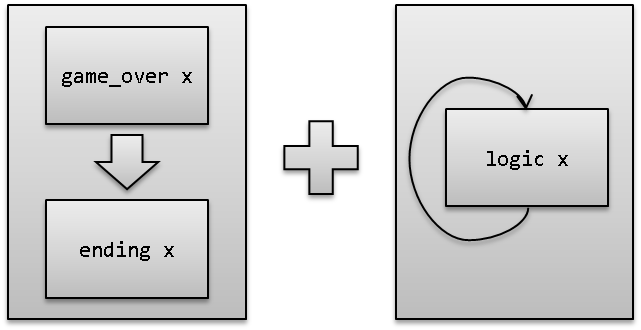
\includegraphics[scale=0.5]{visual_script.png}
\label{Visual script}
\end{center}
 

\section{Conclusions}
\label{sec:conclusions}
%%%%%%%%%%%%%%%%%%%%%%%%%%%%%%%%%%%%%%%%%%%%%%%%%%%%%%%%%%
% conclusions.tex
%%%%%%%%%%%%%%%%%%%%%%%%%%%%%%%%%%%%%%%%%%%%%%%%%%%%%%%%%%

Scripts are an important and pervasive aspect of computer games. Scripts simplify the interaction with computer game engines to the point that a designer or an end-user can easily customize gameplay. Scripting languages must support coroutines because these are a very recurring pattern when creating gameplay modules. Scripts should be fast at runtime because games need to run at interactive framerates. Finally, the scripting runtime should be as modular and as programmable as possible to facilitate its integration in an existing game engine.

In this paper we have shown how to use meta-programming facilities (in particular monads) in the functional language F\# to enhance the existing scripting systems which are based on Lua, the current state of the art, in terms of speed, safety and extensibility. We have also shown how having a typed representation of coroutines promotes building powerful libraries of combinators that abstract many common patterns found in scripts. As evidence of the capabilities of our proposed system we have outlined a series of applications of our scripts into an actual game that is under development.
 
% 1 pages

\vfill\eject

\bibliographystyle{plain}
\bibliography{references} 
% 0 pages

\end{document}
